\documentclass[english]{article}
\usepackage[english]{babel} 
\usepackage[T1]{fontenc}
\usepackage[utf8x]{inputenc}
\usepackage{float}
\usepackage{graphicx}

\makeatletter
\usepackage[a4paper,top=2cm,bottom=2cm,left=2cm,right=2cm]{geometry}
\usepackage{enumitem}
\usepackage{subfig}
\usepackage{amsthm}
\usepackage{amsmath}
\usepackage{epstopdf}
\usepackage{fancyhdr}
\usepackage{booktabs,array}
\usepackage{graphicx}

\hyphenation{english}
\makeatother

\usepackage{babel}


\usepackage{listings}
\usepackage{xcolor} % for setting colors

% set the default code style
\lstset{
	frame=tb, % draw a frame at the top and bottom of the code block
	tabsize=4, % tab space width
	showstringspaces=false, % don't mark spaces in strings
	numbers=left, % display line numbers on the left
	commentstyle=\color{gray}, % comment color
	keywordstyle=\color{blue}, % keyword color
	stringstyle=\color{red} % string color
}

\begin{document}
	\begin{titlepage}
		
		\begin{center}
			\begin{Large} \textbf{UNIVERSITY OF PADOVA} \\
			\end{Large} \vspace{1cm}
			\vspace{3cm}
			\begin{Large} Embedded Real--Time Control \end{Large}
			\par\end{center}
		
		\begin{center}
			\begin{Large}Laboratory report\\
			\end{Large}
			\par\end{center}
		
		\begin{center}
			\vspace{2cm}
			\begin{figure}[!htb]
				\centering \includegraphics[width=8cm]{figures/unipd-logo.png}\\
				
			\end{figure}
			
			\par\end{center}
		
		\begin{center}
			\vspace{2cm}
			\begin{Large} Moamen Mohamed Abouelabbas - 2159249  \\
			\end{Large}
			\begin{Large} Kiavash Rabbani Soudabi - 2141822  \\
			\end{Large} \vspace{2cm}
			\begin{Large} Academic Year 2024-2025 \end{Large}
			\par\end{center}
		
	\end{titlepage}
	\tableofcontents
	\newpage
	
	% ==================[ LAB 1]
	\section{Lab 1: Line sensor and	keypad}
	Purpose of this lab is to learn how to interact with an external device, connected to the micro-controller using serial communication.
	
	\subsection{Relevant theoretical notions}
	The primary device used is the \textbf{sx1509}, a GPIO expander that facilitates easy I/O expansion via a standard 400kHz I2C interface. It is particularly useful in scenarios where the microcontroller has a limited number of I/O pins or where remote serial communication is needed.\\
	The TurtleBot employs two sx1509 devices: one connected to a keypad at I2C address $0x3F$, and the other connected to a line sensor at address $0x3E$. For the keypad, data acquisition is handled through an external interrupt triggered on pin PF4.\\
	The keypad is configured as a $4 \times 4$ matrix, with each row and column connected to specific GPIO pins of the sx1509 (referred to as sx1509\_2). The state of each key is stored in two registers: REG\_KEY\_DATA\_1 (for columns) and REG\_KEY\_DATA\_2 (for rows).\\
	
	\begin{figure}[!htb]
		\centering 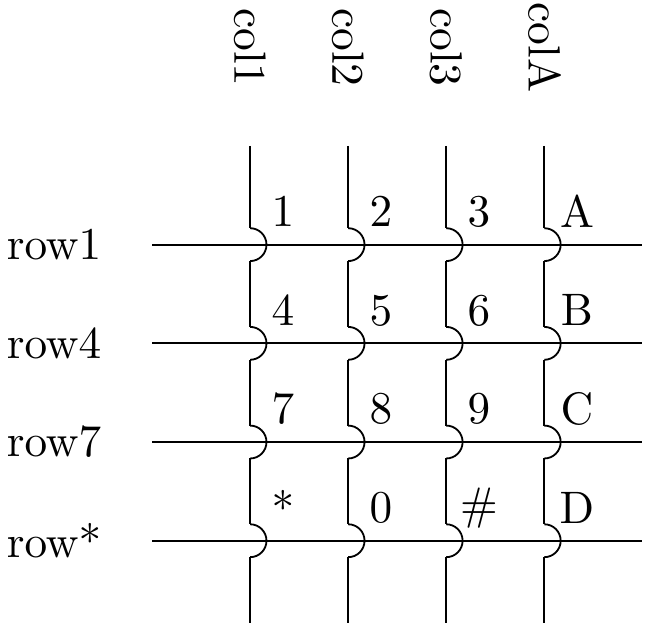
\includegraphics[width=6cm]{figures/Keypad_connection.png}\\
		\caption{Keypad connection schema}		
	\end{figure}
	
		% ================== Section: Exercise 1 ==================
	\subsection{Exercise 1: Handling Keypad Interrupts}
	Write an ISR that recognizes and correctly handles the keypad interrupts and  read the registers REG\_KEY\_DATA\_1
	and REG\_KEY\_DATA\_2 inside the ISR.\\
	This exercise is done inside the \texttt{HAL\_GPIO\_EXTI\_Callback(uint16\_t pin)} which is a callback function provided by the STM32 HAL (Hardware Abstraction Layer) library. It is called automatically whenever a GPIO external interrupt (EXTI) is triggered.\\
	\subsubsection{Code Contribution}
	\begin{lstlisting}[language=C, caption={Keypad interrupt handler}, breaklines=true]
		if (GPIO_Pin == GPIO_PIN_4) { // Check if interrupt is from PF4
			uint8_t key_data_1, key_data_2;
			
			// Read the keypad column data
			if (HAL_I2C_Mem_Read(&hi2c1, SX1509_I2C_ADDR2 << 1, REG_KEY_DATA_1, I2C_MEMADD_SIZE_8BIT, &key_data_1, 1, 100) != HAL_OK) {
				printf("Error reading REG_KEY_DATA_1\n");
				return;
			}
			
			// Read the keypad row data
			if (HAL_I2C_Mem_Read(&hi2c1, SX1509_I2C_ADDR2 << 1, REG_KEY_DATA_2, I2C_MEMADD_SIZE_8BIT, &key_data_2, 1, 100) != HAL_OK) {
				printf("Error reading REG_KEY_DATA_2\n");
				return;
			}
			
			// Print the detected key status
			printf("Interrupt triggered on PF4\n");
			printf("Keypad column data: 0x%02X\n", key_data_1);
			printf("Keypad row data: 0x%02X\n", key_data_2);
		}
	\end{lstlisting}
	
	\subsubsection{Console Output}
	\begin{lstlisting}[caption={Output}]
		Interrupt on pin (16).
		Keypad column data: 0xFE
		Keypad row data: 0xF7
		...
	\end{lstlisting}
	
	\subsubsection{Notes}
	No configuration was required beyond what's prewritten. Interrupts were used as required.\\
	
	% ================== Section: Exercise 2 ==================
	\subsection{Exercise 2: Decoding Keypad Input}
	Print which keypad button has been
	pressed.\\
	
	\subsubsection{Code Contribution}
	The following code reads the keypad column and row data and decode it to the pressed key. Moreover, it returns \texttt{"?"} if the data is not valid.
	\begin{lstlisting}[language=C, caption={Key decoding routine}, breaklines=true]
		const char keypad[4][4] = {
			{'1', '2', '3', 'A'},
			{'4', '5', '6', 'B'},
			{'7', '8', '9', 'C'},
			{'*', '0', '#', 'D'}
		};
		
		// Exercise2: Function to get key from register values
		char decode_key(uint8_t col_data, uint8_t row_data) {
			int row = -1, col = -1;
			
			// Identify row
			switch (row_data) {
				case 0xFE: row = 3; break;  // Row 1 (bit 0 changed)
				case 0xFD: row = 2; break;  // Row 2 (bit 1 changed)
				case 0xFB: row = 1; break;  // Row 3 (bit 2 changed)
				case 0xF7: row = 0; break;  // Row 4 (bit 3 changed)
			}
			
			// Identify column
			switch (col_data) {
				case 0xFE: col = 0; break;  // Column 1
				case 0xFD: col = 1; break;  // Column 2
				case 0xFB: col = 2; break;  // Column 3
				case 0xF7: col = 3; break;  // Column 4
			}
			
			// Return the corresponding key if valid row and column detected
			if (row != -1 && col != -1) {
				return keypad[row][col];
			}
			
			return '?';  // Unknown key
		}
		
		// Decode and print the key
		char key = decode_key(key_data_1, key_data_2);
		if (key != '?') {
			printf("Keypad column data: 0x%02X\n", key_data_1);
			printf("Keypad row data: 0x%02X\n", key_data_2);
			printf("Key Pressed: %c\n", key);
		} else {
			printf("Unknown key press detected\n");
		}
	\end{lstlisting}
	
	\subsubsection{Console Output}
	\begin{lstlisting}[caption={Output}]
		Interrupt on pin (16).
		Keypad column data: 0xFE
		Keypad row data: 0xF7
		Key Pressed: 1
		Interrupt on pin (16).
		Keypad column data: 0xFD
		Keypad row data: 0xF7
		Key Pressed: 2
		...
	\end{lstlisting}
	
	\subsubsection{Notes}
	In this section, an issue was encountered with the configuration of the row data pins, which were actually set in the opposite order relative to the column data pins. As a result, the output did not correctly reflect the pressed key. After several iterations of trial and error, the correct pin configuration was identified and implemented.\\
	
	% ================== Section: Exercise 3 ==================
	\subsection{Exercise 3: Line Sensor Data via Polling}
	Write a routine that reads the status of the line sensor and prints it. The routine must check the status with a polling period of 100ms.\\
	\subsubsection{Code Contribution}
	In this part, the line sensor data is read through the I2C bus, and a function is implemented to convert the sensor’s original hexadecimal output into a more readable binary format that clearly represents the system’s 8-sensor array.\\
	
	\begin{lstlisting}[language=C, caption={Polling-based line sensor readout}, breaklines=true]
		void printBinary(uint8_t num) {
			for (int i = 7; i >= 0; i--) {
				printf("%d", (num >> i) & 1);  // Extract each bit
				if (i % 4 == 0) printf(" ");  // Add space for readability
			}
			printf("\n");
		}
		
		while (1)
		{
			/* USER CODE END WHILE */
			HAL_Delay(100);
			uint8_t lineSensorData;   
			
			// Exercise3: Read the status of line sensor
			if (HAL_I2C_Mem_Read(&hi2c1, SX1509_I2C_ADDR1 << 1, REG_DATA_B, 1, &lineSensorData, 1, I2C_TIMEOUT) != HAL_OK) {
				printf("Error reading REG_DATA_B\n");
				return 0;
			}
			
			printf("Line sensor data (BIN): ");
			printBinary(lineSensorData);
		}
	\end{lstlisting}
	
	\subsubsection{Console Output}
	\begin{lstlisting}[caption={Output}]
		Line sensor data (BIN): 11111111
		Line sensor data (BIN): 11101111
		...
	\end{lstlisting}
	
	\subsubsection{Notes}
	Using binary printouts made interpreting sensor status much easier. Initially unclear outputs were clarified through this strategy.
	
	% ================== Section: Exercise 4 ==================
	\subsection{Exercise 4: Frequency-Controlled LED (Bonus)}
	 Making one of the LED blink with dynamic frequency using the keypad input.\\
	 
	\subsubsection{Code Contribution}
	The following code implements the process of receiving a frequency input and converting it into a corresponding delay time for LED blinking.
	
	\begin{lstlisting}[language=C, caption={Input-driven LED toggle},breaklines=true]
		// Global variables
		char inputBuffer[MAX_DIGITS + 1] = {0};  // Buffer to store user input
		int myindex = 0;  // Tracks number of entered digits
		int frequency = 0;
		
		// Inside the interrupt handler after decoding the pressed key
		if (key >= '0' && key <= '9') {
			if (myindex < MAX_DIGITS) {
				inputBuffer[myindex++] = key;  // Store digit
			}
		} 
		else if (key == '#') {  // End input on `#`
			inputBuffer[myindex] = '\0';  // Null-terminate string
			frequency = atoi(inputBuffer);  // Convert to integer
			printf("\nEntered frequency: %d Hz\n", frequency);
			
			// Reset buffer for next input
			memset(inputBuffer, 0, sizeof(inputBuffer));
			myindex = 0;
		}
		
		
		// Inside the while loop
		if (frequency != 0) {
			uint32_t delayTime = 1000 / (2 * frequency);
			HAL_Delay(delayTime);
			HAL_GPIO_TogglePin(GPIOE, GPIO_PIN_5);
		}
	\end{lstlisting}
	
	\subsubsection{Console Output}
	\begin{lstlisting}[caption={Output}]
		Entered frequency: 1 Hz		
		Entered frequency: 2 Hz		
		Entered frequency: 100 Hz
		...
	\end{lstlisting}
	
	\subsubsection{Notes}
	Implemented the bonus version with input parsing. LED toggled reliably. This was one of the more technically engaging tasks.	
	
	
	% ======================= Lab 2 ay
	\section{Lab 2: Open loop control}
	The purpose of this lab is to implement an open loop camera stabilizer using the IMU and servo motors.\\
	\subsection{Relevant theoretical notions}
	IMU stands for Inertial Measurement Unit. It's a device that uses a combination of sensors to measure and report an object's acceleration, angular rate (rotation), and sometimes the magnetic field surrounding it.
	
	\subsection{Exercise 1: Tilt Stabilization Using IMU-Based Control Law}
	The tilt angle $\theta$ of the TurtleBot, representing rotation around the x-axis, can be estimated using the y-axis output of the onboard accelerometer. Assuming the robot is stationary or moving slowly, the dominant force measured is gravity, allowing orientation to be inferred.\\
	The angle is computed using the following expression:\\	
	 \begin{equation}
	 	\theta = \arcsin(\frac{a_y}{g})	 
	 \end{equation}
	 where $a_y$ is the measured acceleration along the y-axis, and $g=9.81m/s^2$ is the gravitational constant. This equation derives from the projection of the gravitational vector onto the sensor’s y-axis.
	 
	\subsubsection{Code Contribution}
	The first step involves acquiring the appropriate measurement from the IMU. The IMU operates at a sampling frequency of 100 Hz, which corresponds to a 20 ms delay within the main execution loop.To access the sensor data, the function \texttt{bno055\_convert\_double\_accel\_xyz\_msq()} is used, which converts the raw accelerometer readings from the BNO055 sensor into double-precision floating-point values representing acceleration.\\
	It is important to note that the output of the inverse sine function used to calculate the tilt angle is in radians; however, the servo control logic requires this value to be expressed in degrees. The control gain is set to -1, ensuring that the camera counteracts the tilt motion of the robot.\\
	Although the \texttt{\_\_HAL\_TIM\_SET\_COMPARE} includes an internal call to the \texttt{saturate()} function to prevent the PWM signal from exceeding safe limits, applying an additional saturation layer introduces no harm and may provide an extra level of safety.\\After logging the relevant data for analysis and debugging, the servo control signal is computed using the following expression:\\
	
	\begin{equation}
		150+camera\_tilt\times (\frac{50.0}{45.0})
	\end{equation}
	
	This formula linearly maps the camera tilt angle (in degrees) to a corresponding PWM compare value. A tilt of \(0^\circ\) results in a neutral PWM value of 150. A full positive tilt of \(+45^\circ\) maps to 200, and a full negative tilt of \(-45^\circ\) maps to 100.\\
	
	
	 
	
	
	\begin{lstlisting}[language=C, caption={Tilt Stabilization},breaklines=true]
		while (1)
		{
			/* USER CODE END WHILE */
			
			/* USER CODE BEGIN 3 */
			HAL_Delay(20);
			bno055_convert_double_accel_xyz_msq(&d_accel_xyz);
			bno055_convert_double_gyro_xyz_rps(&d_gyro_xyz);
			
			// Read the y acceleration data
			y_accelerate = d_accel_xyz.y;
			
			// calculate tilt angle
			float g = 9.81; // m/s^2
			tilt = asin(y_accelerate / g) * (180 / M_PI); // convert to degrees
			camera_tilt = -tilt;
			
			// limit the tilt to 45 to -45
			if(camera_tilt > 45) camera_tilt = 45;
			if(camera_tilt < -45) camera_tilt = -45;
			
			//update data logger value
			logger_data.y_accelerate = y_accelerate;
			logger_data.tilt_angle = (float)tilt;			
			ertc_dlog_update(&logger); // check if someone is connected and waiting for data
			ertc_dlog_send(&logger, &logger_data, sizeof(logger_data)); // send data
			
			
			/* update pan-tilt camera */
			__HAL_TIM_SET_COMPARE(&htim1, TIM_CHANNEL_2,
			(uint32_t)saturate((150+camera_tilt*(50.0/45.0)), SERVO_MIN_VALUE, SERVO_MAX_VALUE)); 
		}
	\end{lstlisting}
	
	\subsubsection{Output}
	\begin{figure}[!htb]
		\centering 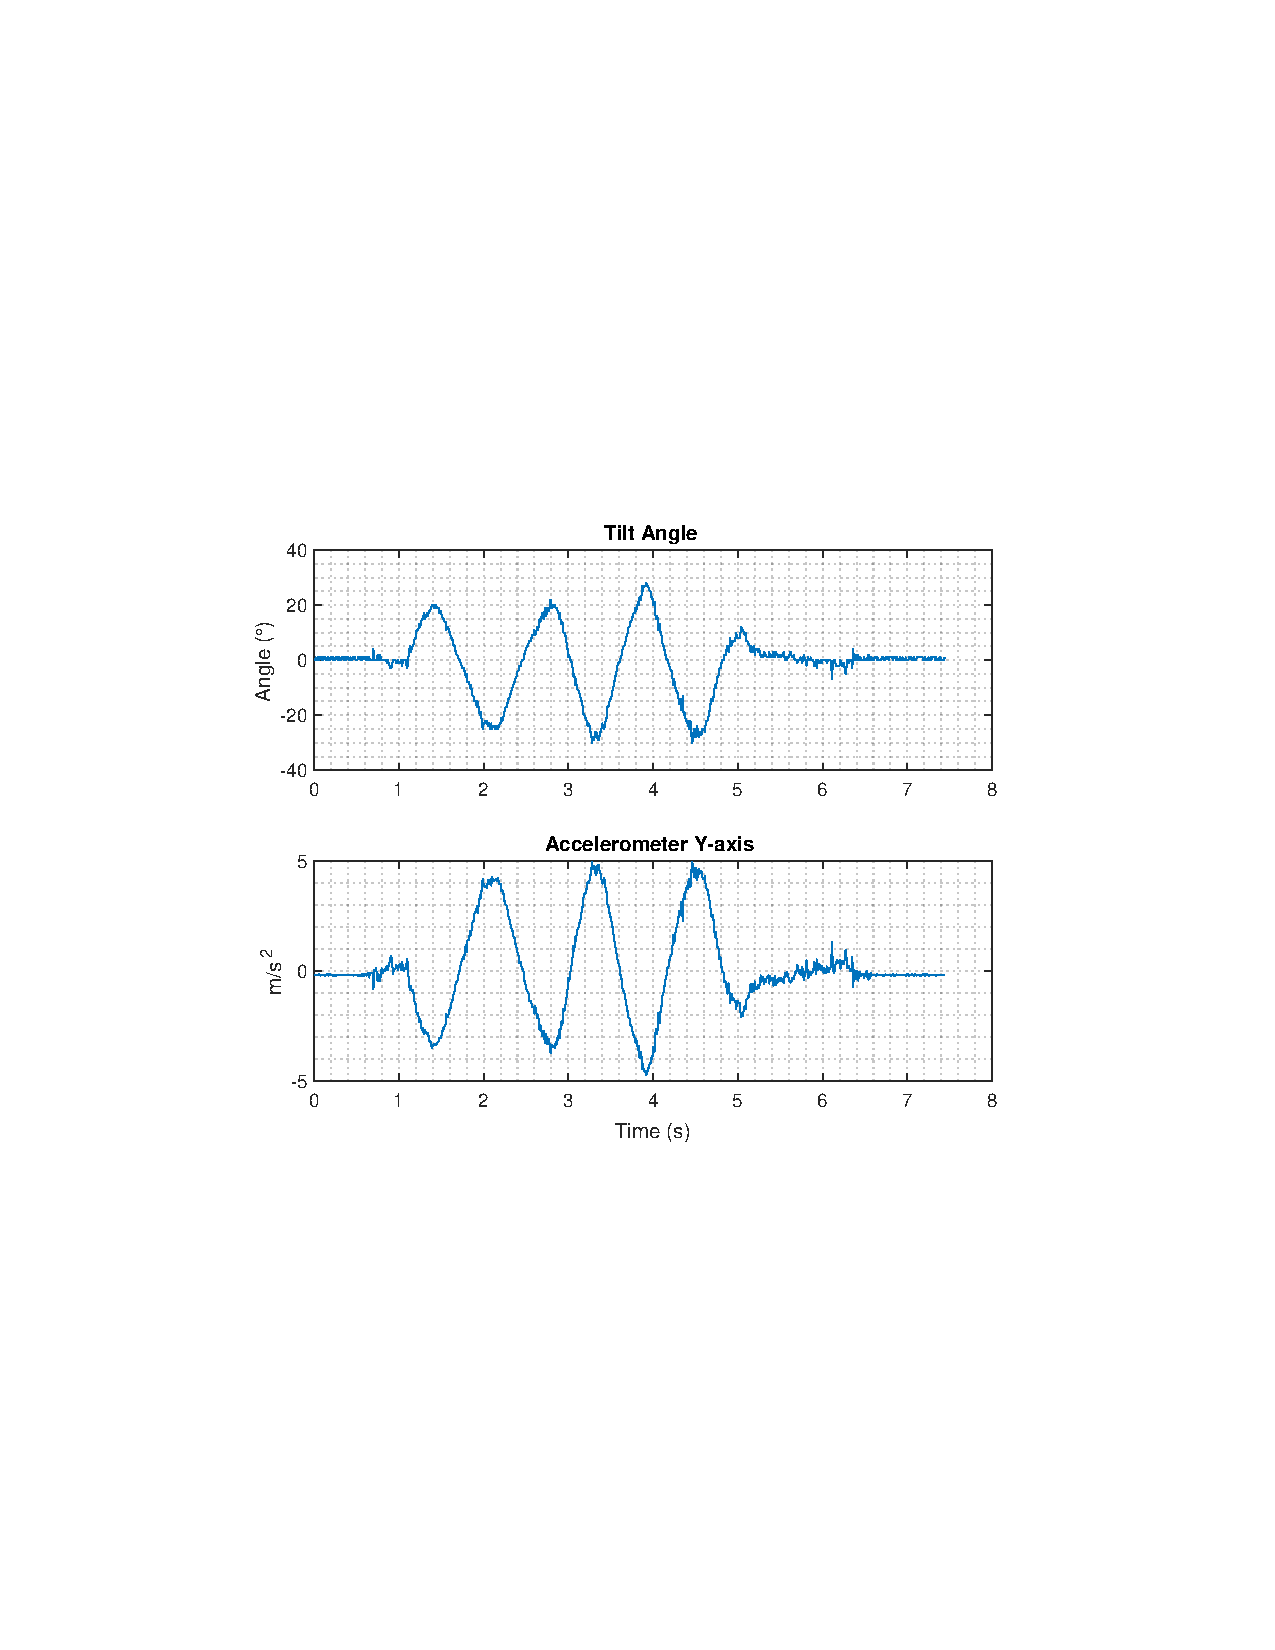
\includegraphics[width=10cm]{figures/lab2ex1output}\\
		\caption{Keypad connection schema}		
	\end{figure}
	
	\subsection{Bonus 1: Gyroscope-Based Smooth Pan Control}
	\subsection{Bonus 2: Sensor Fusion for Enhanced Tilt/Pan Control}
	
\end{document}
